\documentclass[a4paper,twoside,13pt]{extbook}
\usepackage[inner=2cm,outer=2cm,top=2cm,bottom=2cm]{geometry}
\usepackage{amssymb,amsmath,amsthm,mathtools}
\usepackage[utf8]{vietnam}
\usepackage{indentfirst}
\usepackage{titlesec}
\usepackage{graphicx}
\usepackage{multirow}
\usepackage{caption}
\usepackage{subfiles}

\setcounter{secnumdepth}{4}
\graphicspath{{IMAGE/}}



\begin{document}
\chapter{PHÂN TÍCH ĐỘNG LƯỢNG PHẦN TỬ CÁNH CHONG CHÓNG}

Trong phần này, chúng ta sẽ trình bày mô hình được đề xuất bởi Glauert để mô tả tương tác giữa turbine và dòng chảy. Sau khi giới thiệu các biến biến số liên quan, chúng ta sẽ đi qua các phép suy luận để dẫn đến các phương trình của mô hình. Sau đó chúng ta sẽ đi vào chi tiết hai phiên bản cảu mô hình được xét.

\section{Các biến số}

Lý thuyết động lựơng phần tử cánh có mục tiêu là thiết lập các quan hệ đại số mà nó đặc trưng cho tương tác giữa lưu chất và một cánh chong chóng đang xoay, từ đây về sau, chúng ta sẽ gọi nó là turbine. Theo hướng này, mô hình của Glauert sẽ kết hợp hai mô tả : một mô hình vĩ mô toàn cục mô tả sự phát triển của các vòng lưu chất đi qua tuabin và một mô hình cục bộ của tuabin, mà nó tóm tắt 2D hoạt động của một phần cánh chong chóng, \emph{một phần tử cánh chonh chóng}, dưới tác dụng của lưu chất.

Dòng chảy được cho là không đổi theo thời gian và không nén được. Tính không nén được ngụ ý rằng vận tốc dòng chảy trong các vùng lân cận bên trái và bên phải của tuabine có cùng giá trị $U_0$. Chúng ta kí hiệu vận tốc dòng thượng nguồn và dòng hạ nguồn lần lượt là $U_{-\infty}$ và $U_{+\infty}$. Mặc dù không được nói đến trong chương này, chúng ta có thể xét đến vận tốc tiếp tuyến có thể được nghiên cứu. Đặc biệt, một bước nhảy của các biến do đĩa truyền động thường được báo cáo và có thể được mô hình hóa bởi trong khuôn khổ của lý thuyết động lượng. Bởi vì mô hình không tính đến tương tác giữa các phần của cánh chong chóng và giả sử rằng $\Omega$ và $U_{\infty}$ là hằng số, chúng ta xét trong chương này một phần tử cánh chong chóng cố định và \emph{tỉ số tốc độ địa phương} cố định $\displaystyle\lambda := \frac{\Omega r}{U_{-\infty}}$. Trong đó, $r$ là khoảng cách từ phần tử đến trục xoay, với $r\le R$, trong đó $R$ là bán kính của cánh chong chóng. Trong các trường hợp thực tế, turbine hoạt động với \emph{tốc độ mũi cánh hằng số (TSR)} : $\Omega$ được điều khiển thông qua moment xoắn do máy phát tạo ra theo cách sao cho $\displaystyle\lambda := \frac{\Omega r}{U_{-\infty}}$ được giử cố định đối với các giá trị khác nhau của ${U_{-\infty}}$. Do đó $\lambda r$ chỉ  phụ thuộc vào $r$. Trong phần tiếp theo, chúng tôi sử dụng biến $\lambda r$ để mô tả vị trí của phần tử cánh chong chóng.

\subsection{Các biến vĩ mô và các mô hình BEM chưa được biết}

Mô hình của Glauert bao gồm một hệ ba biến $a$, $b$ và $\varphi$ liên kết với nhau đối với một vòng lưu chất. Hai số đầu tiên được gọi là \emph{số hạng cảm ứng trục} và \emph{số hạng cảm ứng góc}. Chúng được định nghĩa bởi :
\begin{equation}\label{eq:1_1}
    \begin{aligned}
        a:=\frac{U_{-\infty}-U_0}{U_{-\infty}}, \qquad b:=\frac{\omega}{2\Omega}.
    \end{aligned}
\end{equation}
trong đó $\omega$ là tốc độ quay của vòng lưu chất. Góc $\varphi$ được gọi là \emph{góc lệch tương đối} của vòng, có nghĩa là :
\begin{equation}\label{eq:1_2}
    \begin{aligned}
        \tan \varphi  = \frac{{1 - a}}{{{\lambda _r}\left( {1 + b} \right)}}.
    \end{aligned}
\end{equation}

Vì mục đích đơn giản và để nhấn mạnh vai trò ẩn số trong mô hình Glauert,
chúng ta bỏ qua sự phụ thuộc của $a$, $b$, $\varphi$ (và $\alpha$) theo $\lambda_r$ trong ký hiệu.
\subsection{Các biến địa phương}

Chúng ta hãy kí hiệu $U_{rel}$ là vận tốc tương đối của lưu chất (cũng
gọi là vận tốc biểu kiến của lưu chất) nhận được từ phần tử cánh chong chóng này khi quay. Theo định nghĩa của $\varphi$, chúng ta có:
\begin{equation}\label{eq:1_3}
    \begin{aligned}
        {U_{rel}} = \frac{{{U_0}}}{{\sin \varphi }}
    \end{aligned}
\end{equation}

Biến này không được xác định khi $\varphi=0$ và như là một đại lượng trung gian, sẽ không xuất hiện trong mô hình cuối cùng. Tuy nhiên, trường hợp giới hạn $\varphi=0$ được thảo luận trong Phần 2.4. Đối với một cấu hình cánh chong chóng nhất định, hệ số lực nâng và lực cản $C_L$ và $C_D$ được xác định bởi :
\begin{equation}\label{eq:1_5}
    \begin{aligned}
        dL = {C_L}\left( \alpha  \right)\frac{1}{2}\rho U_{rel}^2{c_{{\lambda _r}}}dr,\qquad dD = {C_D}\left( \alpha  \right)\frac{1}{2}\rho U_{rel}^2{c_{{\lambda _r}}}dr,
    \end{aligned}
\end{equation}
trong đó $\rho$ là khối lượng riêng của lưu chất, $dL$ và $dD$ là nguyên tố lực nâng và lực cản tác dụng lên phần tử cánh chong chóng có độ dày $dr$ và độ dài dây cung cánh $c_{\lambda}$. Tham số $\alpha$ được gọi là \emph{góc tấn} và được định nghĩa là góc giữa dây cung cánh và hướng dòng chảy, 
do đó thỏa mãn mối quan hệ :
\begin{equation}\label{eq:1_6}
    \begin{aligned}
        \alpha  = \varphi  - \gamma_{\lambda _r},
    \end{aligned}
\end{equation}
trong đó $- \pi /2 < \gamma {\lambda _r} < \pi /2$ là \emph{góc xoắn} của cánh chong chóng. Các thông số liên quan đến phần tử cánh chong chóng được tóm tắt trong Hình 1.1.
\begin{figure}[h!]
	\centering
	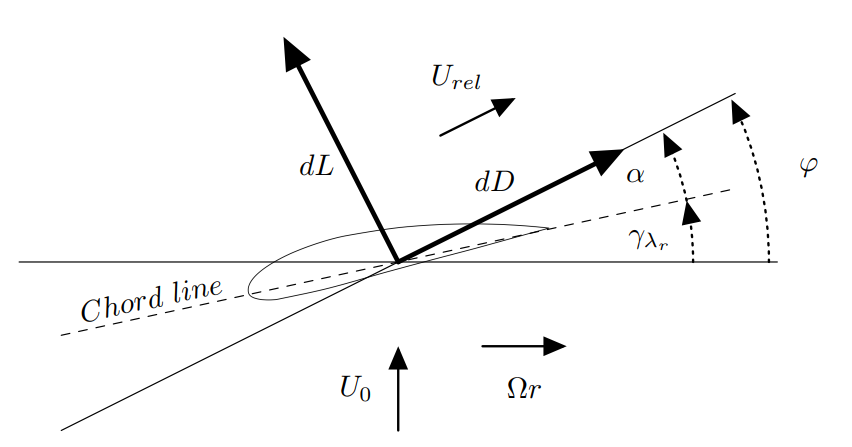
\includegraphics[scale=0.75]{BLADE_PROFILE.png}
	\caption{Biên dạng phần tử cánh chong chóng và các góc, vận tốc và lực liên quan.}
\end{figure}

Hệ số $C_L$ và $C_D$ tương ứng với tỷ số giữa lực nâng và lực cản với lực động, tức là lực liên kết với động năng quan sát được. Chúng được xác định bởi biên dạng của cánh chong chóng. Sau khi điều này được cố định, các tham số thiết kế chính là $c_{\lambda_r}$ và $\gamma_{\lambda_r}$ mà sự tối ưu hóa được thảo luận trong Phần 5.

Các hệ số $C_L$ và $C_D$ được giả sử là hàm của $\alpha$ và thỉnh thoảng của số Reynolds ($Re$). Trường hợp phụ thuộc vào số Reynold hiếm khi được xem xét trong các sách chuyên khảo, trong đó Re được giả định là không đổi đối với $\alpha$ khi $U_{\infty}$, $\lambda_r$, $\Omega$, $c_{\lambda_r}$ là cố định. Để đơn giản, chúng tôi cũng bỏ qua những thay đổi của $Re$ trong chương này. Tuy nhiên, kết quả của chúng tôi có thể được mở rộng cho trường hợp số Reynolds không phải hằng số, tức là trong các tình huống mà các hàm $\left( {\alpha ,{\mathop{\rm Re}\nolimits} } \right) \mapsto {C_L}\left( {\alpha ,{\mathop{\rm Re}\nolimits} } \right)$
và $\left( {\alpha ,{\mathop{\rm Re}\nolimits} } \right) \mapsto {C_D}\left( {\alpha ,{\mathop{\rm Re}\nolimits} } \right)$ phải được tính đến. Trong thực tế, $Re$ được giả định là được biết trước và được sử dụng để chọn $C_L$ và $C_D$, hoặc xử lý lặp đi lặp lại cùng với $C_L$ và $C_D$ để có được kết quả chính xác hơn.

Mặc dù thay đổi từ profile này sang profile khác, các hành vi của $C_L$ và $C_D$ theo $\alpha$ có thể được mô tả một cách định tính theo một cách tổng quát. Hệ số $C_L$ thường tăng gần như tuyến tính đối với $\alpha$ đến một góc tới hạn $\alpha_s$ cho trước, với $0 < {\alpha _s} < \pi /2$, mà ở đó xảy ra hiện tượng stall: $C_L$ giảm nhanh chóng, gây mất lực nâng đột ngột. $C_D$ liên kết với một lực cản, nó luôn luôn dương và xác định với mọi góc. Hệ số thường tăng nhẹ với $\alpha$ lên đến giá trị $\alpha=\alpha_s$, và sau đó trở nên rất lớn. Mặc dù hầu hết các thiết kế không ngăn phần bên trong của cánh chong chóng tạo ra stall, điều kiện $\varphi  - {\gamma _{{\lambda _r}}} < {\alpha _s}$ thường được xem xét trong giai đoạn thiết kế cánh chong chóng. Ghi chú cuối cùng là phần lớn phân tích của chúng tôi áp dụng cho các góc tấn sao cho $C_L$ dương. Các thuộc tính của $C_L$ và $C_D$ cần thiết cho phân tích của chúng tôi được tóm tắt trong giả thiết sau đây.\\

\textsc{Giả thiết 1}. \textit{Cho $\beta\in\mathbb{R}^+$, hàm $\alpha \mapsto {C_L}\left( \alpha  \right)$ liên tục trên ${I_\beta }: = \left[ { - \beta ,\beta } \right]$, và dương trên ${I_\beta } \cap \mathbb{R}^+$. Hàm số $\alpha  \mapsto {C_D}\left( \alpha  \right)$ được xác định, liên tục và không âm trên $\mathbb{R}$.}\\

Do đó, $C_L(0)$ được giả định là dương, trong thực tế nó là tương đương với góc tấn không có lực nâng là âm. Giả định này là đúng cho các thiết kế thông thường.
\section{Mô hình Glauert}
Vì lý do sự đầy đủ, bây giờ chúng tôi nhớ lại lý do do Glauert đề xuất để lập mô hình tương tác giữa tuabine và một dòng chảy. Chúng tôi kí hiệu $dT$ và $dQ$ lần lượt là lực đẩy và moment xoắn vô cùng nhỏ trên phần tử cánh chong chóng có độ dày $dr$ đang được xem xét.
\subsection{Phương pháp tiếp cận vĩ mô}
Phần đầu tiên của mô hình liên quan đến lý thuyết động lượng và đề cập đến sự tiến hóa vĩ mô của một vòng chất lỏng. Nó được dùng để biểu diển $dT$ và $dQ$ theo $a$,$a_0$ và $\varphi$.

Chúng ta kí hiệu $p_-$ và $p_+$ lần lượt là áp suất chất lỏng ở các vùng lân cận bên trái và bên phải của cánh chong chóng. Áp dụng định luật Bernoulli giữa $-\infty$ và $0^-$ và giữa $0^+$ và $+\infty$ cho chúng ta : ${p_ - } - {p_ + } = \frac{1}{2}\rho \left( {U_{ - \infty }^2 - U_{ + \infty }^2} \right)$. Chúng ta xem xét tốc độ thay đổi động lượng ở cả hai phía của tuabine, chúng tôi nhận được biểu thức thứ hai đối với sự biến thiên của áp suất, cụ thể là ${p_ - } - {p_ + } = \rho \left( {{U_{ - \infty }} - {U_{ + \infty }}} \right){U_0}$. Kết hợp hai phương trình trước và sử dụng , chúng ta thu được ${U_{ + \infty }} = \left( {1 - 2a} \right){U_{ - \infty }}$. Vì $dT = \left( {{p_ - } - {p_ + }} \right)2\pi rdr$ và $dQ = \omega \rho {U_0}2\pi {r^3}dr$, chúng ta có :
\begin{equation}\label{eq:1_7}
    \begin{aligned}
            dT = {C_T}\left( a \right)U_{ - \infty }^2\rho \pi rdr,
    \end{aligned}
\end{equation}
\begin{equation}\label{eq:1_8}
    \begin{aligned}
            dQ = 4b\left( {1 - a} \right){\lambda _r}{U_0}\rho \pi {r^2}dr.
    \end{aligned}
\end{equation}

Trong đó $\displaystyle {C_T}\left( a \right): = \frac{{dT}}{{\frac{1}{2}U_{ - \infty }^2\rho 2\pi rdr}} = 4a\left( {1 - a} \right)$, là \emph{hệ số lực đẩy địa phương}.
\subsection{Phương pháp tiếp cận cục bộ}
Một nhóm các phương trình khác có thể nhận được thông qua lý thuyết phần tử cánh chong chóng, trong đó các biểu thức cục bộ cho lực đẩy và moment xoắn vô cùng nhỏ được xét đến. Việc suy luận bao gồm việc kết hợp nguyên tố lực nâng và lực cản (2.4) được diển giải trong tham chiếu quay với (2.3). Điều này cho chúng ta :
\begin{equation}\label{eq:1_9}
    \begin{aligned}
        dT = {\sigma _{{\lambda _r}}}\frac{{{{\left( {1 - a} \right)}^2}}}{{{{\sin }^2}\varphi }}\left( {{C_L}\left( \alpha  \right)\cos \varphi  + {C_D}\left( \alpha  \right)\sin \varphi } \right)U_{ - \infty }^2\rho \pi rdr
    \end{aligned}
\end{equation}
\begin{equation}\label{eq:1_10}
    \begin{aligned}
        dQ = {\sigma _{{\lambda _r}}}\frac{{{{\left( {1 - a} \right)}^2}}}{{{{\sin }^2}\varphi }}\left( {{C_L}\left( \alpha  \right)\sin \varphi  - {C_D}\left( \alpha  \right)\cos \varphi } \right)U_{ - \infty }^2\rho \pi rdr,
    \end{aligned}
\end{equation}
trong đó $\displaystyle{\sigma _{{\lambda _r}}}: = \frac{{B{c_{{\lambda _r}}}}}{{2\pi r}}$, với $B$ là số lượng cánh của turbine.
\subsection{Kết hợp phươnh pháp toàn cục và cục bộ}
Để có được một hệ thống các phương trình đóng hơn, Glauert kết hợp các kết quả của hai khảo sát. Chính xác hơn, tương ứng, cân bằng (2,6) và (2,7) với (2,8) và (2,9), sử dụng (2,5) và chia cả hai phương trình kết quả của $4 (1 - a)^2$ cho ta :
\begin{equation}\label{eq:1_11}
    \begin{aligned}
        \frac{a}{{1 - a}} = \frac{{{\sigma _{{\lambda _r}}}}}{{4{{\sin }^2}\varphi }}\left( {{C_L}\left( {\varphi  - {\gamma _{{\lambda _r}}}} \right)\cos \varphi  + {C_D}\left( {\varphi  - {\gamma _{{\lambda _r}}}} \right)\sin \varphi } \right),
    \end{aligned}
\end{equation}
\begin{equation}\label{eq:1_12}
    \begin{aligned}
        \frac{b}{{1 - a}} = \frac{{{\sigma _{{\lambda _r}}}}}{{4{\lambda _r}{{\sin }^2}\varphi }}\left( {{C_L}\left( {\varphi  - {\gamma _{{\lambda _r}}}} \right)\sin \varphi  - {C_D}\left( {\varphi  - {\gamma _{{\lambda _r}}}} \right)\cos \varphi } \right).
    \end{aligned}
\end{equation}

Hệ phương trình thu được bằng cách kết hợp (2.2), (2.10) và (2.11) là cơ sở của lý thuyết động lượng phần tử cánh chong chóng.
\section{Mô hình đơn giản}
Trong các chuyên khảo khí động học turbine, các tác động của $C_D$ đôi khi được bỏ qua. Chúng ta sẽ thảo luận điều này về sau.

Giả định này thực sự được chứng minh trong nhiều trường hợp, vì các quy trình thiết kế cố gắng giảm thiểu tối đa lực cản. Trong thực tế, quy trình thiết kế lưỡi dao thông thường bắt đầu bằng cách chọn góc xoắn $\gamma_{\lambda_r}$ tối thiểu tỉ lệ $\displaystyle\frac{C_D}{C_L}$, xem Phần 5.1.

Chúng tôi xem xét trường hợp $C_D = 0$ và gọi chúng là \emph{mô hình đơn giản hóa} trong các phần tiếp theo. Theo các phương trình (2.2), (2.10) và (2.11), nó tương ứng với ba phương trình:
\begin{equation}\label{eq:1_13}
    \begin{aligned}
        \tan \varphi  = \frac{{1 - a}}{{{\lambda _r}\left( {1 + b} \right)}},
    \end{aligned}
\end{equation}
\begin{equation}\label{eq:1_14}
    \begin{aligned}
        \frac{a}{{1 - a}} = \frac{1}{{{{\sin }^2}\varphi }}{\mu _L}\left( \varphi  \right)\cos \varphi ,
    \end{aligned}
\end{equation}
\begin{equation}\label{eq:1_15}
    \begin{aligned}
        \frac{b}{{1 - a}} = \frac{1}{{{\lambda _r}\sin \varphi }}{\mu _L}\left( \varphi  \right),
    \end{aligned}
\end{equation}
trong đó chúng tôi đã giới thiệu hàm vô thứ nguyên $\displaystyle{\mu _L}\left( \varphi  \right): = \frac{{{\sigma _{{\lambda _r}}}}}{4}{C_L}\left( {\varphi  - {\lambda _{{\lambda _r}}}} \right)$ được xác định trên ${I_{\beta ,{\gamma _{{\lambda _r}}}}}: = \left[ { - \beta  + {\gamma _{{\lambda _r}}},\beta  + {\gamma _{{\lambda _r}}}} \right]$; theo giả thiết 1.
\section{Mô hình đúng}
Để tiến đến gần hơn với kết quả thực nghiệm, mô hình (2.2,2.10,2.11) cần phải được điều chỉnh. Sau đây, chúng tôi trình bày ba hiệu chỉnh quan trọng, gồm việc cho hệ số cản $C_D$ khác không, hiệu chỉnh mất ở đầu cánh và sự điều chỉnh chuyên biệt cho giá trị lớn của $a$. Cái đầu tiên và cái cuối cùng sẽ điều chỉnh đáng kể việc phân tích được phát triển cho mô hình đơn giản hóa.
\subsection{Lực cản tăng chậm}

Ngoài việc coi $C_D$ hoàn toàn dương, chúng tôi sẽ giả định trong một số phần của phân tích, sự gia tăng chậm của tham số này từ 0 đến khi xảy ra hiện tượng stall.
\subsection{Điều chỉnh mất ở đuôi}

Các phương trình của lý thuyết động lượng được suy ra từ giả định rằng tuabine có thể được mô hình hóa như một đĩa truyền động. Một khuôn khổ như vậy tương ứng với một rotor có vô số cánh quạt. Tuy nhiên, trong các tình huống thực tế, khi điều chỉnh dòng chảy ở đuôi cánh chong chóng phải tính đến sự lưu thông của lưu chất xung quanh cánh chong chóng phải giảm (theo hàm mũ) đến không khi $r\rightarrow R$, với $R$ là bán kính của tuabine. Bằng cách này, Glauert đã giới thiệu một phương pháp gần đúng của hàm đuôi của Prandtl $F_{\lambda_r}$ :
$$
{F_{{\lambda _r}}}\left( \varphi  \right): = \frac{2}{\pi }\arccos \left( {\exp \left( { - \frac{{B/2\left( {1 - \frac{{{\lambda _r}{U_{ - \infty }}}}{{\Omega R}}} \right)}}{{\left( {\frac{{{\lambda _r}{U_{ - \infty }}}}{{\Omega R}}} \right)\sin \varphi }}} \right)} \right) = \frac{2}{\pi }\arccos \left( {\exp \left( { - \frac{{B/2\left( {1 - r/R} \right)}}{{\left( {r/R} \right)\sin \varphi }}} \right)} \right)
$$
như một yếu tố bổ sung cho (2.6) và (2.7). Sự sửa đổi này làm phát sinh :
\begin{equation}\label{eq:1_16}
    \begin{aligned}
        dT = 4a\left( {1 - a} \right){F_{{\lambda _r}}}\left( \varphi  \right)U_{ - \infty }^2\rho \pi rdr,
    \end{aligned}
\end{equation}
\begin{equation}\label{eq:1_17}
    \begin{aligned}
        dQ = 4b\left( {1 - a} \right){F_{{\lambda _r}}}\left( \varphi  \right)U_{ - \infty }^2\rho \pi {r^3}\Omega dr.
    \end{aligned}
\end{equation}

Lưu ý rằng một số tác giả chỉ đưa hệ số mất ở đuôi vào trong (2.6). Kết quả
của chương này của chúng tôi có thể dễ dàng được điều chỉnh cho phù hợp với phiên bản này của mô hình. Hơn nữa, các mô hình sửa chữa sự mất mát ở đuôi đã được giới thiệu. Một cách tiếp cận thay thế dựa trên việc mở rộng lý thuyết xoáy.
\subsection{Điều chỉnh cho các giá trị lớn của $a$}
Đối với hệ số cảm ứng lớn hơn 0.4, wake rối thường xuất hiện, và người ta chấp nhận rộng rãi rằng lý thuyết động lượng không áp dụng được. Sự thật này đã được báo cáo bởi Glauert, người đã đề xuất sửa đổi $C_T (a)$ trong (2.6) khi $a$ trở nên lớn hơn hơn một ngưỡng $a_c$ nhất định. Sau đó, nhiều biểu thức đã được đề xuất để phù hợp hơn với dữ liệu thử nghiệm. Tất cả các biến thể này dẫn đến một biểu thức mới cho $dT$ :
\begin{equation}\label{eq:1_18}
    \begin{aligned}
        dT = 4\left( {a\left( {1 - a} \right) + \psi \left( {{{\left( {a - {a_c}} \right)}_ + }} \right)} \right){F_{{\lambda _r}}}\left( \varphi  \right)U_{ - \infty }^2\rho \pi rdr.
    \end{aligned}
\end{equation}
trong đó $(a-a_c)_+ := \text{max}\{0,a-a_c\}$ và là một hàm xác định trên $\mathbb{R}^+$. Một số hiệu chỉnh được trình bày thông qua hàm trong Bảng 1. Hiệu chỉnh theo kinh nghiệm của Glauert thu được bằng cách kết hợp dữ liệu thực nghiệm và các ràng buộc $C_T(a_c) = 4a_c(1-a_c)$ và $C_T (1) = 2$. Điều này dẫn đến sự gián đoạn tại $a = a_c$ khi $F_{\lambda_r}(\varphi)\ne 1$. Buhl đề xuất một điều chỉnh để khắc phục vấn đề này.
\begin{table}[h!]
    \centering
        \begin{tabular}{|c ||c |c|} 
        \hline
            Tác giả & $a_c$ & $\psi((a-a_c)_+)$ \\ [0.5ex] 
            \hline\hline
            Glauert & 1/3 & $\frac{{{{\left( {a - {a_c}} \right)}_ + }}}{4}\left( {\frac{{\left( {a - {a_c}} \right)_ + ^2}}{{{a_c}}} + 2{{\left( {a - {a_c}} \right)}_ + } + {a_c}} \right)$ \\
            \hline
            Công thức bán thực nghiệp Glauert & 2/5 & $\approx \left( {\frac{1}{{2\left( {1 - {a_c}} \right)}} - \frac{\nu }{4}\left( {1 - a} \right)} \right){\left( {a - {a_c}} \right)_ + } \text{ với }\nu = 5.5563$ \\
            \hline
            Buhl & 2/5 & $\frac{1}{{2{F_{{\lambda _r}}}\left( \varphi  \right)}}{\left( {\frac{{{{\left( {a - {a_c}} \right)}_ + }}}{{1 - {a_c}}}} \right)^2}$ \\
            \hline
            Wilson, Spera & 1/3 & $\left( {a - {a_c}} \right)_ + ^2$ \\ [1ex] 
    \hline
    \end{tabular}
    \captionof{table}{Các hiệu chỉnh khác nhau có thể được đưa ra liên quan đến hệ số lực đẩy và hệ số cảm ứng (2.15) trong trường hợp trạng thái rối.} 
\end{table}


\subsection{Về các hiệu ứng 3D}

Để tính đến các tác động của hiệu ứng 3D khi cánh chonh chóng xoay, chúng ta có thể áp dụng các công thức được hiệu chỉnh cho mô hình. Chúng ta có thể xét như một ví dụ, công thức hiệu chỉnh sau đây :
\[C_L^c = {C_L} + a{\left( {\frac{{{c_{{\lambda _r}}}}}{r}} \right)^b}\Delta {C_L}\]
trong đó $a\in[2,3]$ và $b\in[1,2]$ là hằng số $\delta C_L=C_{L,inv}-C_L$. $C_{L,inv}$ là hệ số lực nâng thu được khi giả thiết lưu chất là không nhớt. Ta cũng dùng một biểu thức tương tự đối với $C_D$. Vì lý do đơn giản, chúng tôi không xem xét hiệu ứng 3D, nhưng tất cả các kết quả sau
có thể dễ dàng điều chỉnh bằng cách thay thế $C_L$ và $C_D$ bằng các biểu thức đã hiệu chỉnh của chúng, như được thực hiện trong phần tiếp theo với sự mất mát ở đuôi.
\subsection{Hệ phương trình đã điều chỉnh}
\begin{equation}\label{eq:1_19}
    \begin{aligned}
        \tan \varphi  = \frac{{1 - a}}{{{\lambda _r}\left( {1 + b} \right)}},
    \end{aligned}
\end{equation}
\begin{equation}\label{eq:1_20}
    \begin{aligned}
        \frac{a}{{1 - a}} = \frac{1}{{{{\sin }^2}\varphi }}\left( {\mu _L^c\left( \varphi  \right)\cos \varphi  + \mu _D^c\left( \varphi  \right)\sin \varphi } \right) - \frac{{\psi \left( {{{\left( {a - {a_c}} \right)}_ + }} \right)}}{{{{\left( {1 - a} \right)}^2}}},\\
    \end{aligned}
\end{equation}
\begin{equation}\label{eq:1_21}
    \begin{aligned}
        \frac{b}{{1 - a}} = \frac{1}{{{\lambda _r}{{\sin }^2}\varphi }}\left( {\mu _L^c\left( \varphi  \right)\sin \varphi  - \mu _D^c\left( \varphi  \right)\cos \varphi } \right),
    \end{aligned}
\end{equation}
trong đó chúng ta đã giới thiệu hàm vô thứ nguyên $\mu _L^c\left( \varphi  \right): = \frac{{{\sigma _{{\lambda _r}}}}}{{4{F_{{\lambda _r}}}\left( \varphi  \right)}}{C_L}\left( {\varphi  - {\gamma _{{\lambda _r}}}} \right)$ và $\mu _D^c\left( \varphi  \right): = \frac{{{\sigma _{{\lambda _r}}}}}{{4{F_{{\lambda _r}}}\left( \varphi  \right)}}{C_D}\left( {\varphi  - {\gamma _{{\lambda _r}}}} \right)$
\section{Phân tích mô hình Glauert và sự tồn tại nghiệm}

Trong phần này, chúng tôi thu gọn từng phiên bản trong số hai phiên bản trước của mô hình Glauert thành một phương trình vô hướng duy nhất. Với mục tiêu chứng minh sự tồn tại, chúng tôi phải xây dựng các giả thiết liên quan đến đặc tính của tuabin. Để đơn giản hóa ký hiệu, chúng tôi giới thiệu góc $\theta_{\lambda_r} \in (0,\frac{\pi}{2})$ được xác định bởi
\begin{equation}\label{eq:1_22}
    \begin{aligned}
        \tan\theta_{\lambda_r} := \frac{1}{\lambda_r},
    \end{aligned}
\end{equation}
và khoảng 
\begin{equation}\label{eq:1_23}
    \begin{aligned}
        I: = {I_{\beta ,{\gamma _{{\lambda _r}}}}} \cap \left( { - \frac{\pi }{2} + {\theta _{{\lambda _r}}},\frac{\pi }{2} + {\theta _{{\lambda _r}}}} \right),\qquad{I^ + }: = I \cap \left( {0,{\theta _{{\lambda _r}}}} \right]
    \end{aligned}
\end{equation}
\subsection{Mô hình được đơn giản hóa}

\begin{description}
    \item[Định lý 3.1] Giả sử rằng Giả thiế t 1 được nghiệm đúng và $(\varphi,a,b)\in I - \{0,\frac{\pi}{2}\}\times\mathbb{R} -\{1\} \times\mathbb{R}-\{-1\}$ thỏa mãn (2.12-2.14). Thì $\varphi$ thỏa :
    \begin{equation}\label{eq:1_24}
        \begin{aligned}
            \mu_L(\varphi) = \mu_G(\varphi)
        \end{aligned}
    \end{equation}
    trong đó $\mu_G(\varphi):=\sin\varphi\tan(\theta_{\lambda_r}-\varphi)$. Ngược lại, giả sử rằng $\varphi\in$ thỏa mãn (\ref{eq:1_24}) và định nghĩa $a$ và $b$ như là các nghiệm tương đương của (2.13) và (2.14) 
\end{description}
\subsection{Mô hình được hiệu chỉnh}

Chúng ta xét mô hình được định nghĩa chính xác bởi (\ref{eq:1_19}-\ref{eq:1_21}), đối với giá trị $a_c\in(0,1)$. Do đó, để thực hiện tham số hóa mô hình và xết sự tồn tại.\\

\textsc{Bổ đề } Giả sử rằng Giả thiết 1 được nghiệm đúng và định nghĩa, với $\varphi\in I^+$

\end{document}